\section{\heiti 实验}

\subsection{\heiti 实验数据}

实验使用开源的数据集CAIL 2018~\cite{xiao2018cail2018largescalelegaldataset},共涵盖1927685个案例,覆盖202种刑事罪名和 183 条刑法法规,其中训练集有1927685条数据,测试集有216829;在数据集中,多被告案件法条分布往往存在长尾分布现象。如图\ref{fig:acc_dis}所示各个法条在判决结果中的出现频率及其占比有较大的不同.在测试数据的法条分布中,占比最高的5个罪行是,盗窃,危险驾驶,故意伤害和交通肇事,其占比分别达到了20.63\%,17.17\%,10.49\%,8.29\%,7.33\%;占比最高的10种罪行占总测试数据的73.58\%。而占比最少的100种罪行只占到总数据的1.83\%。
\begin{figure}[H]
		\centering
		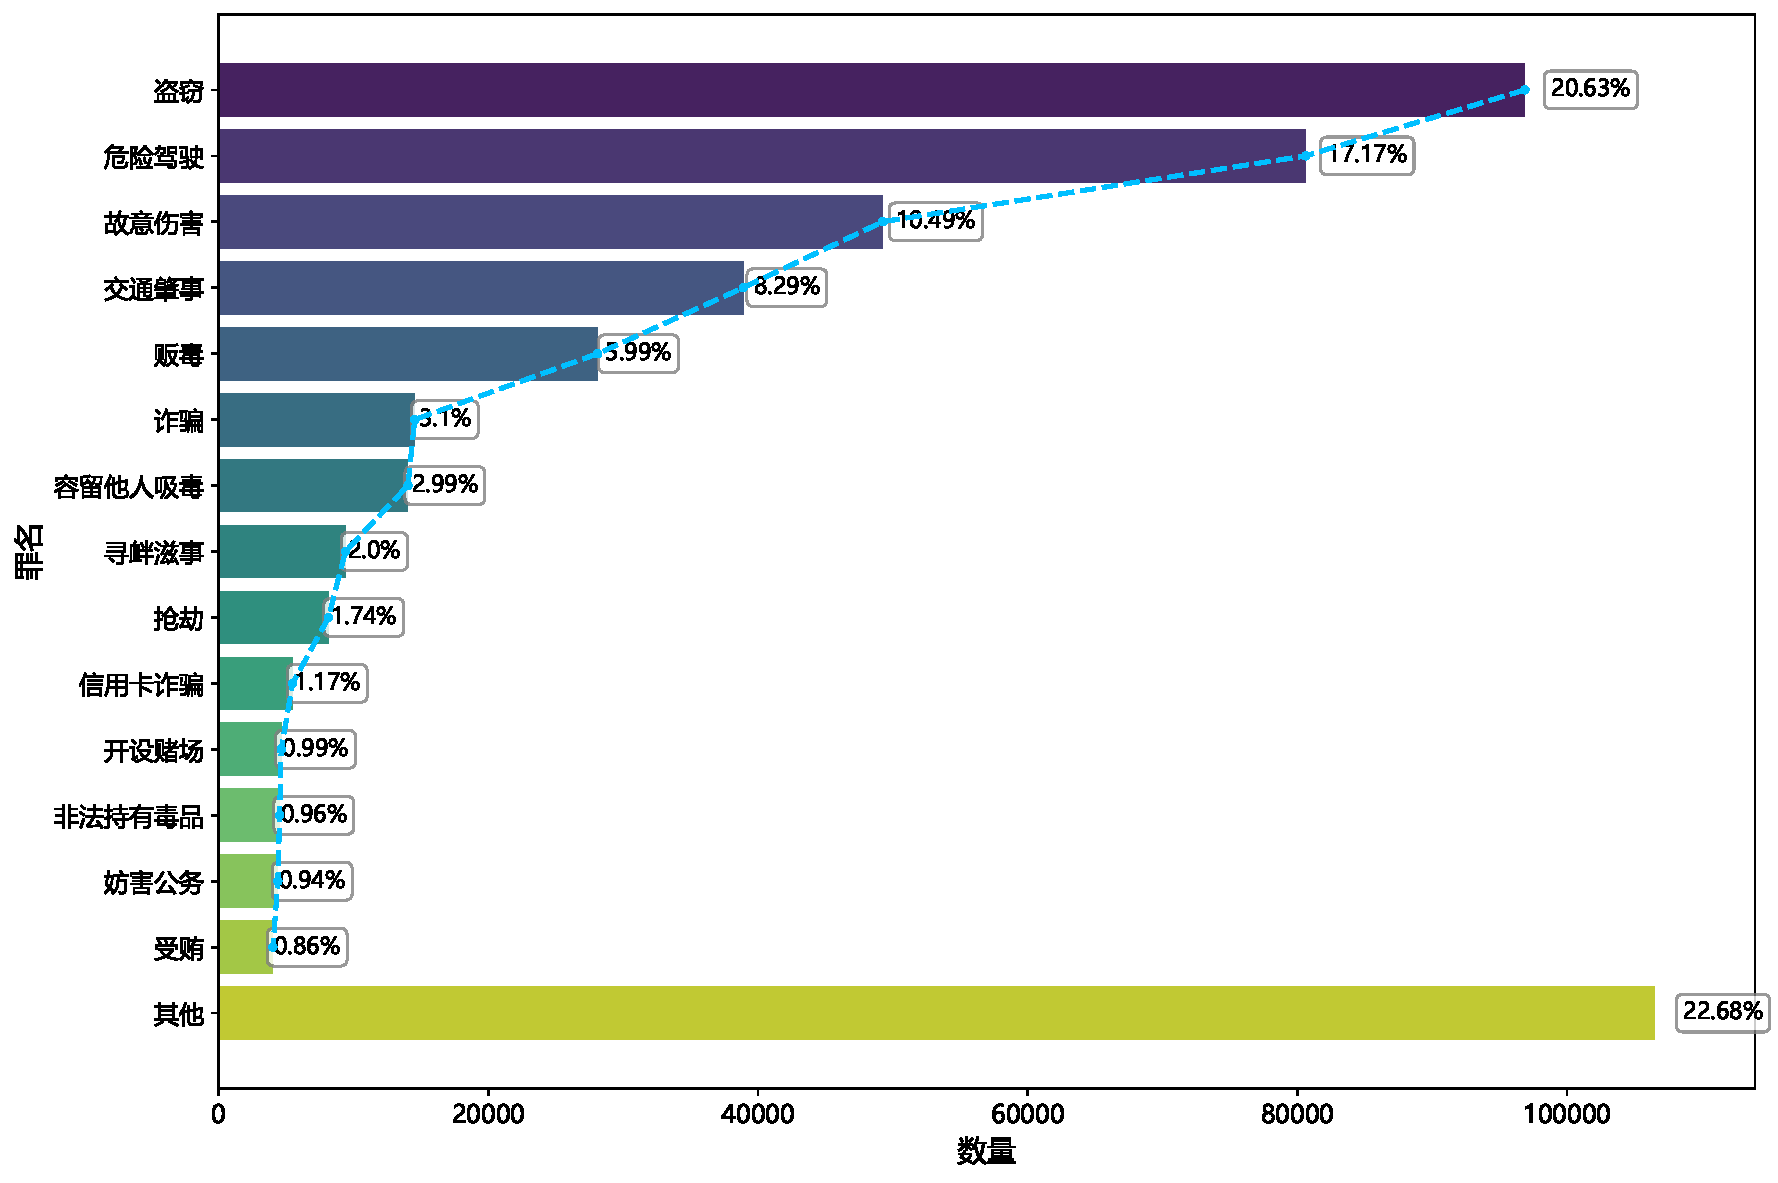
\includegraphics[width=1\linewidth]{fig/accusation_distribution.pdf}
		\caption{测试数据的罪名分布}
		\label{fig:acc_dis}
\end{figure}
如图\ref{fig:art_dis}法条数据分布也呈现长尾趋势。占比最高的10种相关法条占测试数据中0.73\%,而占比最低的100种法条只占2.44\%。
\begin{figure}[H]
    \centering
    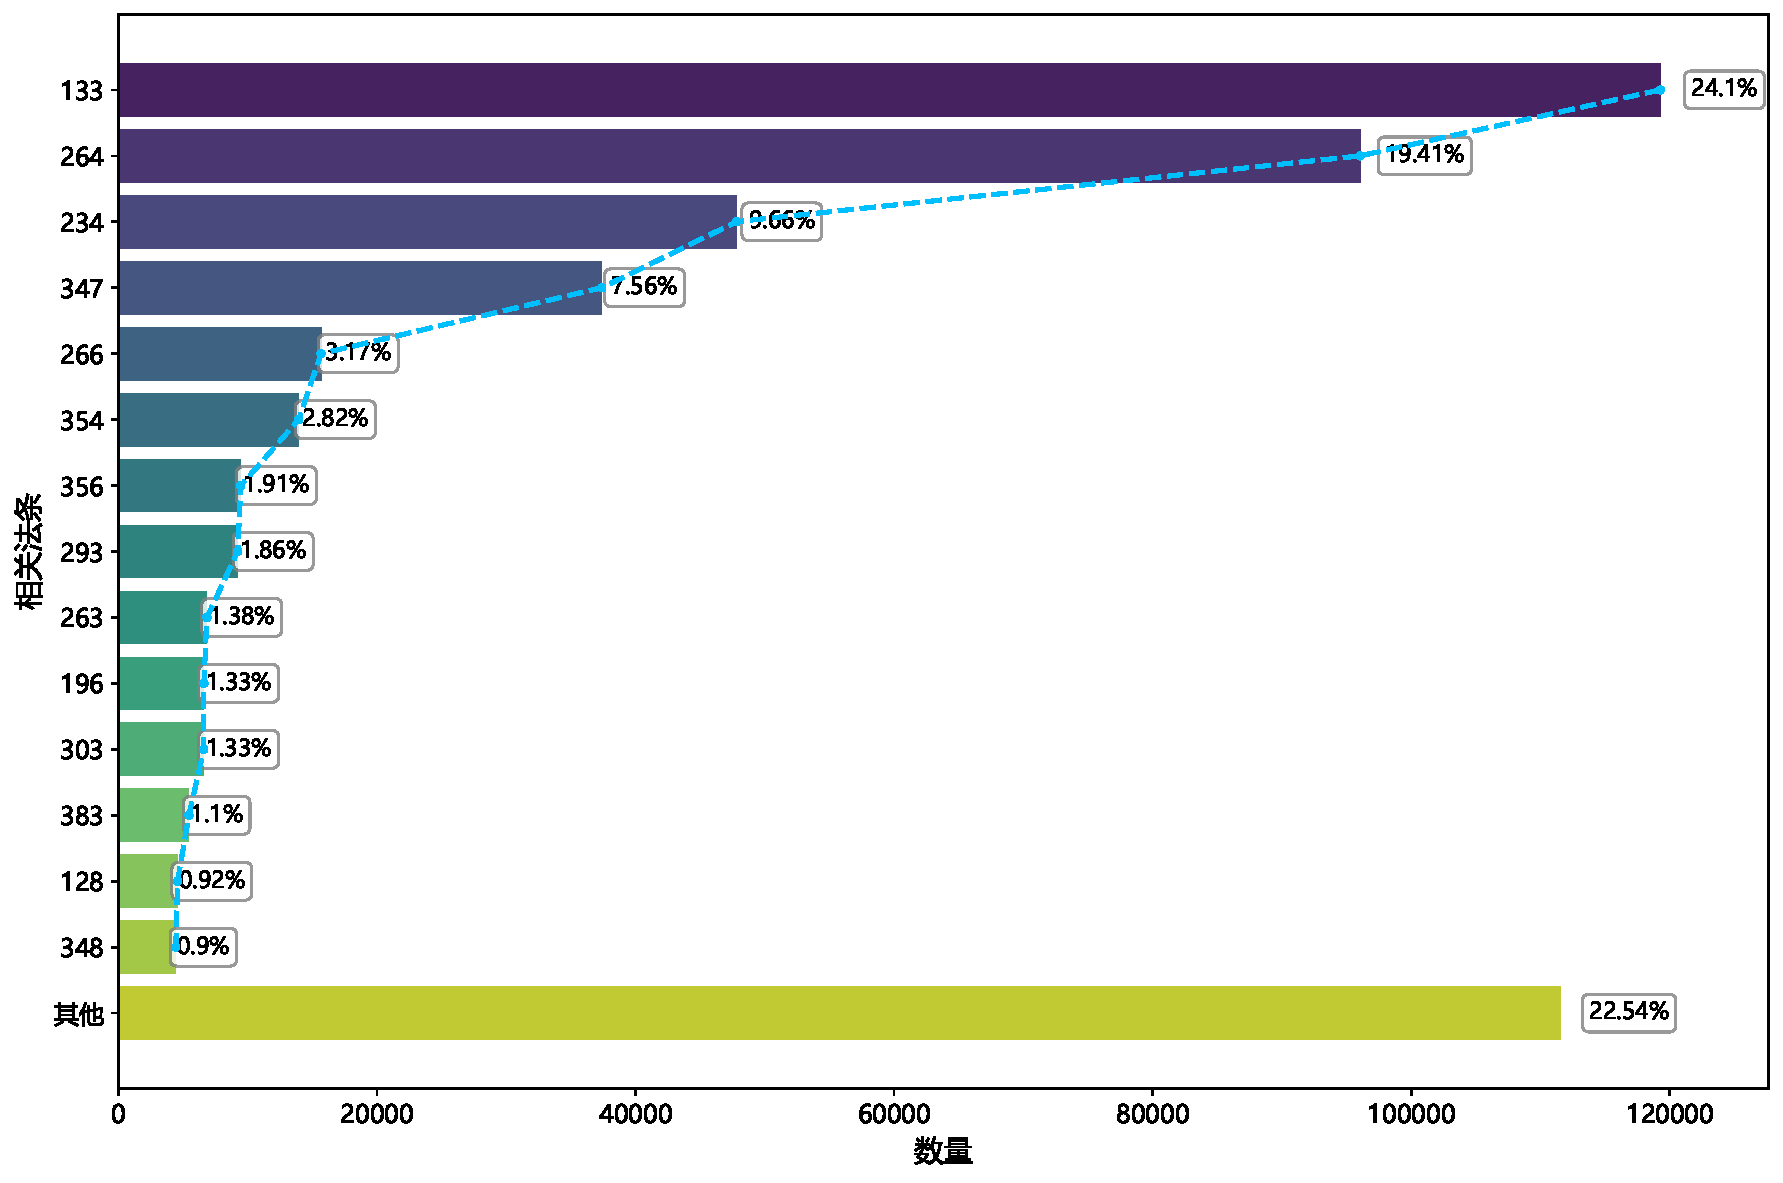
\includegraphics[width=1\linewidth]{fig/article_distribution.pdf}
    \caption{测试数据的法条数据分布}
    \label{fig:art_dis}
\end{figure}
\subsection{\heiti 实验设置}
本研究案例数据库利用CAIL 2018~\cite{xiao2018cail2018largescalelegaldataset}的训练集构造。为了控制案例数据库的大小,平衡检索效率和案例丰富的,本研究从训练集中每种罪名最多抽取100条数据,一共构建1676个案例。
法条数据库使用中国刑法作为文本数据。
案例数据库和法条数据库的文本嵌入模型使用BAAI/bge-m3模型~\cite{chenBGEM3EmbeddingMultiLingual2024};
向量数据库使用milvus~\cite{2022manu,2021milvus},相似度函数使用内积(Inner Product,IP),向量索引方法采用倒排索引(Inverted File,IVF),聚类中心为200个。搜索算法使用暴力搜索(Flat Search,FALT),在每个聚类内部使用相似度函数进行比较。
要素提取模型采用qwen-turbo,判决模型使用qwen-plus模型~\cite{qwenQwen25TechnicalReport2025}。

\subsection{\heiti 评价指标}
CAIL 2018法律判决预测中的罪名、刑期预测两项子任务,都属于多标签的多分类问题~\cite{xiao2018cail2018}。
本研究采用精度(Precision , P) 、召回率(Recall , R) 和 F1分数 3项指标来衡量模型的预测效果。
\begin{eqnarray}
	&P=\frac{\sum_{i=1}^{n}TP_{i}}{\sum_{i=1}^{n}TP_{i}+\sum_{i=1}^{n}FP_{i}}
	\\
	&R=\frac{\sum_{i=1}^{n}TP_{i}}{\sum_{i=1}^{n}TP_{i}+\sum_{i=1}^{n}FN_{i}}
	\\
	&F1=\frac{2\times P\times R}{P+R}
\end{eqnarray}
中,$i$为分类任务中类别的种类;$TP_i$为True Positive,指被正确地划分了类别 $i$ 的样本个数;$FP_i$ 为False Positive,指实际为其他类但被分类器划分为$i$ 类的样本数;$FN_i$ 为False Negative,指实际为 $i$ 类,但是被分类器划分错误的样本数。

\begin{table*}[htbp]
	\centering
	\caption{ 法律判决预测结果的对比}
	\begin{tabular}{lcccccc}
		\toprule
		\textbf{模型} & \multicolumn{3}{c}{\textbf{罪名}} & \multicolumn{3}{c}{\textbf{刑期}}                                                               \\
		\cmidrule(lr){2-4} \cmidrule(lr){5-7}
		            & \textbf{精确率}                    & \textbf{召回率}                    & \textbf{F1分数} & \textbf{精确率} & \textbf{召回率} & \textbf{F1分数} \\
		\midrule
		MTL-Fusion  & 0.6861                          & 0.6911                          & 0.6886        & 0.3512       & 0.3567       & 0.3539        \\
		Lawformer   & 0.6927                          & 0.7082                          & 0.7004        & 0.3581       & 0.3629       & 0.3605        \\
		BERT        & 0.7011                          & 0.7178                          & 0.7094        & 0.4311       & 0.4308       & 0.4309        \\
		LawChatGLM  & 0.7517                          & 0.7478                          & 0.7497        & 0.4712       & 0.4671       & 0.4691        \\
		Ours        & 0.7797                          & 0.7689                          & 0.7743        & 0.5578       & 0.566        & 0.5525        \\
		\bottomrule
	\end{tabular}
	\label{tab:performance_comparison}
\end{table*}

\subsection{\heiti 基准模型}
为检验基座大语言模型的性能和本研究提出的“基于大语言模型, 法律引导的的案例融合方法”的有效性,及其与基于域外语料训练的法律大模型能力相比的优劣,本研究进行了CAIL 2018两个子任务罪名和刑期的对比实验。对比本文模型与4种基线模型的效果差异。
基线模型的选取覆盖基于词嵌入的深度学习模型MTL-Fusion~\cite{zhuopeng-etal-2020-multi}模型、中国司法长文本文书预训练模型Lawformer~\cite{xiao2021lawformer},预训练模型BERT~\cite{fan2022multi}以及 司法数据微调与RAG结合LawChatGLM~\cite{JSJA202505027}。

\subsection{\heiti 实验结果与分析}


表\ref{tab:performance_comparison}的实验结果清晰地揭示了不同技术路径在法律判决预测任务上的性能差异。从传统模型MTL-Fusion、Lawformer到基于预训练的BERT,再到结合了法律知识增强的LawChatGLM,模型的性能在罪名和刑期预测上呈现出稳步提升的趋势。这证明了更强的语义理解能力和外部知识的引入是提升LJP性能的关键。然而,即便是表现最强的基准模型LawChatGLM,其虽然通过检索法律条文提升了罪名预测的准确性,但在更需酌情裁量的刑期预测上表现仍有较大提升空间(F1分数为0.4691),这表明仅依赖成文法条作为外部知识源尚不足以完全捕捉司法实践的复杂性。

本文提出的方法在所有评价指标上均取得了最优表现,尤其在刑期预测任务上实现了关键突破,F1分数达到0.5525,相较于LawChatGLM提升了8.34个百分点。这一显著优势的核心原因在于我们创新的“法律引导的案例融合”框架。该框架不仅通过检索法律条文为罪名判定提供了权威的法律依据,更关键的是,通过引入“相似案例检索”模块,为模型提供了来自真实司法实践的量刑参考。这些相似判例中蕴含的裁判经验和量刑逻辑,有效弥补了成文法条在具体刑期裁量上的模糊性,使得模型的预测更贴近真实的司法裁判思维。实验结果有力地证明,将大语言模型的推理能力与法律条文的规范性指引、相似案例的实践性参考进行深度融合,是构建高精度、高可靠性智能司法判决系统的有效路径。

\subsection{\heiti 案例研究}
\begin{figure*}[htpb]
    \centering
    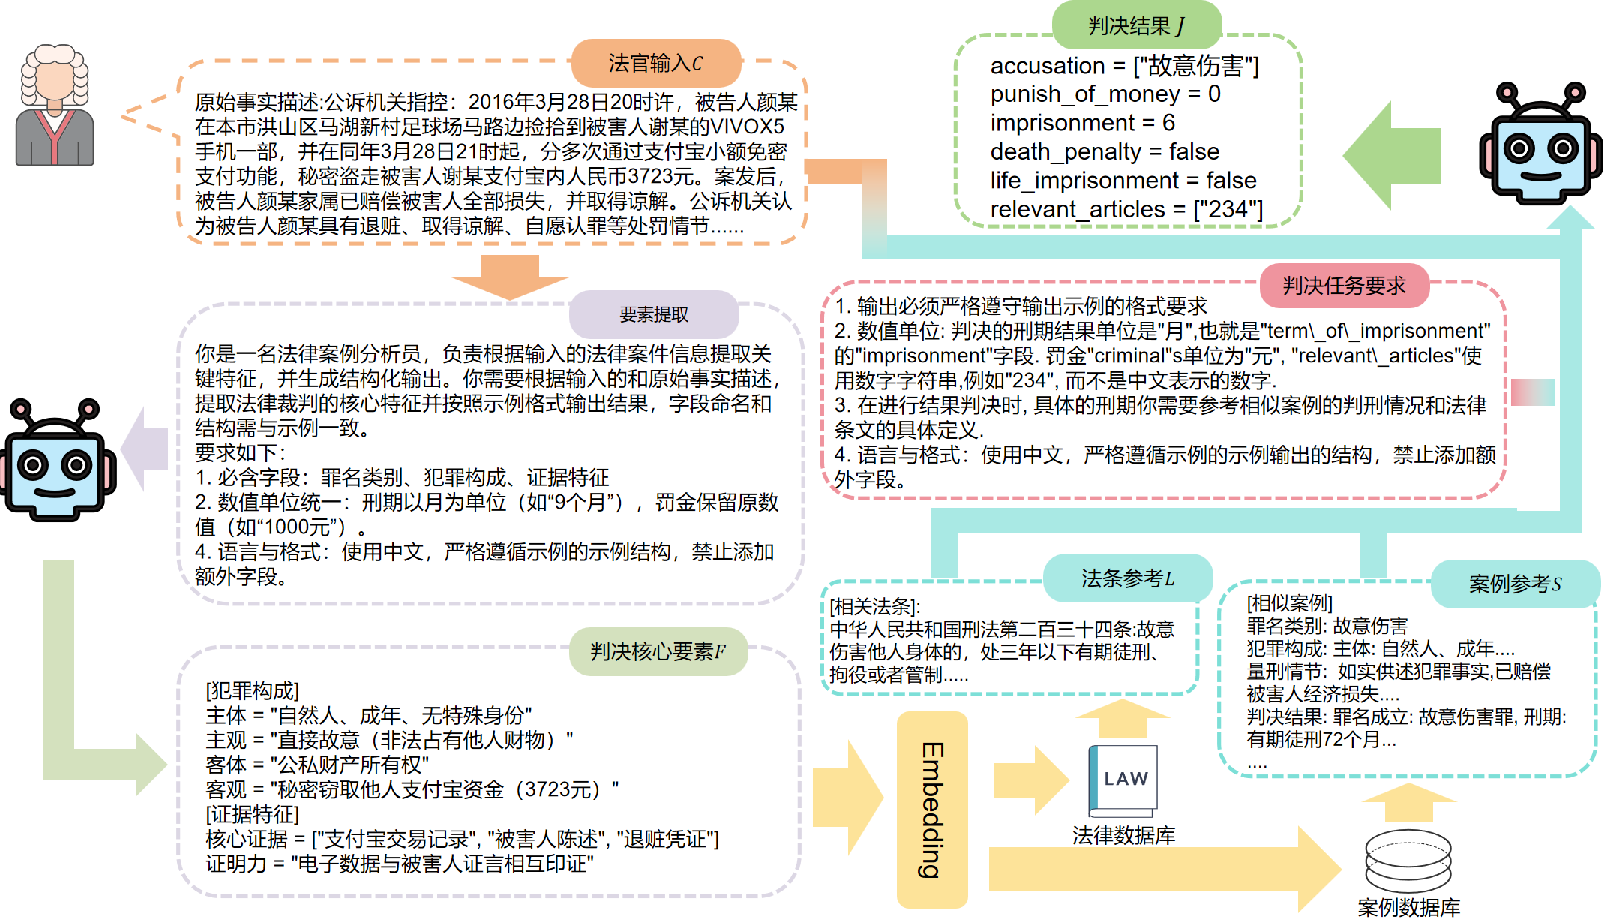
\includegraphics[width=0.8\linewidth]{fig/case.pdf}
    \caption{案例}
    \label{fig:case}
\end{figure*}
本研究提出的方法将以一个具体的盗窃案件为例进行说明。首先,系统接收一段原始的案件事实描述,例如:“公诉机关指控,2016年3月28日20时许,被告人颜某在…盗走被害人谢某支付宝内人民币3723元”。接着,系统利用大语言模型对该文本进行“判决核心要素提取”,生成结构化的犯罪特征($F$),包括犯罪构成(主体、主观、客体、客观)和核心证据等。**随后,进入本方法的核心——双重知识检索阶段。系统会将提取出的核心要素($F$)通过文本嵌入模型(如BAAI/BGE-m3)转换为高维查询向量。该查询向量被用于在两个并行的路径上执行检索:第一条路径中,系统在预先向量化的法律数据库中进行近似最近邻(ANN)搜索,通过计算内积相似度,找出与案件特征最匹配的法律条文($L$),如《中华人民共和国刑法》第二百六十四条;第二条路径中,系统同样利用该查询向量,在向量化的案例数据库中检索相似判例($S$)。此处的案例检索更为精细,它会综合考量罪名、犯罪构成、证据特征等多个维度的相似度,以确保筛选出的历史判例与当前案件具有高度的可比性。**最后,将原始案情($C$)、提取的核心要素($F$)、检索到的法律条文($L$)及相似案例($S$)共同作为输入,送入核心的LLM推理引擎,由其进行综合分析与推理,最终生成一个的结构化判决结果(J):
\\
accusation = ["盗窃罪"]
\\
relevant\_articles = ["264"]
\\
punish\_of\_money = 3723
\\
imprisonment = 7
\\
death\_penalty = false
\\
life\_imprisonment = false

